\chapter{Understanding before building. Variability in analog subthreshold circuits.}
\label{ch:introduction_to_hardware}

The story begins with single spiking neurons and emulation of their behaviour through \ac{MOSFET} transistor physics~\cite{Chicca_etal14}. Before we begin connecitng neurons together, it is essential to have this bottom-layer block well-defined. When implemented in hardware, these circuits are much harder to characterize compared to mathematical models, so let us start with the definition of the spiking neuron model we use. This also will be useful later as we attempt to align the physical neurons with their simulated prototypes and begin seeing the device-induced variability in the behaviour of the similarly tuned silicon neurons.

%With the goal of understanding the brain function through reproduction and knowing that computation is done with networks of these units, it is essential to have this bottom-layer block well-defined. A number of spiking neuron models have been developed with varying levels of complexity and types of biologically relevant behaviour~\cite{Izhikevich04}. Typically, the more complex the model, the more elaborate the dynamics of the real cells it reflects at the cost of additional computational resources. And by resources, one can see not only the calculation steps it takes to solve systems of differential equations but also the physical area it would take to emulate such neuron behaviour with an analog circuit.


\section{Modeling a leaky integrate-and-fire neuron}

Leaky integrate-and-fire (LIF) spiking neuron model is a commonly selected trade-off between biological plausibility and computational complexity. It captures the most essential properties of the biological neurons while remaining fairly accessible for mathematical analysis. LIF neurons are often used in numerical simulations of various SNNs, and are also implemented as transistor circuits on hardware (see the next Section).

From computational neuroscience, the defining behaviour of neuron cells is their ability to integrate electrical pulses (spikes) from dendrites (inputs) and generate action potentials down their axons (outputs) onwards to other neurons.
In neuroinformatics, this is described by different mathematical models with a wide variety of depth and detail~\cite{Izhikevich04}. A common approach is a description of the neuron as a point (i.e. not modelling cell body geometry) and using its membrane potential (or transmembrane voltage) $V_{mem}(t)$ as its state variable.

An optimal trade-off between biological plausibility, computational complexity and analytical interpretability is often seen in the \ac{LIF} neuron model.

\begin{eqnarray}
    \tau_m \frac{dV_{mem}(t)}{dt} & = & - (V_{mem}(t) - V_{rest}) + RI_{in}(t) \label{eq:LIF}\\
    V_{mem}(t) > V_{th} & \rightarrow & V_{mem}(t) = V_{reset}, t^i_{sp} = t
    \label{eq:LIF_reset}
\end{eqnarray}

where in absence of input currents $I_{in}(t)$ though the membrane with conductance $R$, the membrane voltage $V_{mem}$ would decay exponentially to the resting potential $V_{rest}$ with the time constant $\tau_{m}$. The neuron emits a spike if $V_{mem}(t)$ exceeds a threshold value $V_{th}$. In that case, the moment of crossing the threshold $t_{sp}$ is recorded and $V_{mem}(t)$ is reset to $V_{reset}$ for the duration of a refractory period $\tau_{ref}$, after which the dynamics of $V$ is again described by Equation~\ref{eq:LIF}.

With the addition of the spike frequency adaptation and the exponential positive feedback modeling the sodium channels, we get the \ac{ADEXP-LIF} neuron model ~\cite{Brette_Gerstner05} that will be referenced throughout the rest of the work, which in its generalized form is:

\begin{eqnarray}
    \tau_{mem} \frac{dV_{mem}}{dt} & = & - (V_{mem}(t) - V_{rest}) - V_{th}(t) + f(V_{mem}) + R_{m}I_{in}(t)     \label{eq:AdEx}\\
    \tau_{adapt}\frac{dV_{th}(t)}{dt} & = &  -V_{th}(t) + A_{adapt} \delta(t-t_{sp}) \label{eq:LIF_adaptation}\\
    V_{mem}(t) > V_{th} & \rightarrow & V(t) = V_{reset}, t^i_{sp} = t
\end{eqnarray}

where the $f(V_{mem})$ is the exponential positive feedback term, and $V_{th}$ has its own decaying dynamics, increasing with every spike the neuron emits, providing negative feedback for $V_{mem}$ (i.e. decreasing excitability). The incoming spikes (emitted by the neuron itself, in this case) at time $t^i_{sp}$ are commonly modeled as delta-functions~\cite{Dayan_Abbott01}.

The input to the neuron is provided through the input current, a sum of the pulses through connections (synapses) coming from the other neurons and the direct input current that could be injected externally:

\begin{equation}
    I_{in}(t) = \sum_{j}I^{ij}_{syn}(t) + I_{dc}(t)
    \label{eq:I_in}
\end{equation}

Synaptic currents are commonly modeled as exponentially relaxating as well, with spikes from other neurons $j$ arriving to the neuron $i$ at times $t^{ij}_{syn}$:

\begin{equation}
    \tau_{syn}\frac{dI_{syn}(t)}{dt} = -I_{syn}(t) + \sum_{j}\delta(t - t^{ij}_{syn}(t))
    \label{eq:I_syn}
\end{equation}

The set of equations above defines neuronal and synaptic transmission. To utilize them within an embedded setting, there has to be some hardware system that does the numerical calculation of these models.
Here, two approaches are possible: digital simulation or emulation by some other physical process.
In the first case, an iterative solver would numerically solve the equations, for example, using Euler or RK3-RK4~\cite{Butcher96, Brette_etal07} methods. The accuracy of the solution would depend on the method and the timestep size of the solver. Typically, since the described model does not have any stochasticity, the results of the simulation would also be deterministic and thus precisely reproducible, which is ideal for any studies of neural network dynamics and its changes created by any smallest perturbations. The drawback of this approach is the computational load that builds up with the number of neurons and synapses simulated simultaneously, as well as with the precision of the numerical solution. This is where classical von Neumann architecture becomes a limiting factor, imposing constraints on the scale of the network, simulation speed relative to real-time, and energy consumption.

The alternative to numerical simulation is direct hardware \emph{emulation}.

\section{Silicon neurons of the DYNAP-SE1 chip}

%\subsection{The computational substrate. Introducing the neurons of DYNAP-SE1.}


For the second approach, the solutions of the equations are \emph{emulated} directly by the electrical circuits. %Exploiting the property of the \ac{MOSFET} transistors, where below the source-to-gate threshold, the diffusion current through the transistor depends exponentially on the gate voltage \dz{which is a nightmare for a traditional electrical engineer OR ADD THIS TO SECTION DISCUSSION}

%\begin{equation}
%    I = I_0 e^{\frac{-V}{\kappa U_t}}
%\end{equation}

%with $\kappa$ and $U_t$ being constant material properties \dz{OF? TBA},
As a result, a circuit of a DPI \ac{ADEXP-LIF} neuron can be constructed~\cite{Livi_Indiveri09, Chicca_etal14}, as illustrated in Figure~\ref{fig:DPI_neuron_and_synapse}.

\begin{figure}[h]
    \centering
    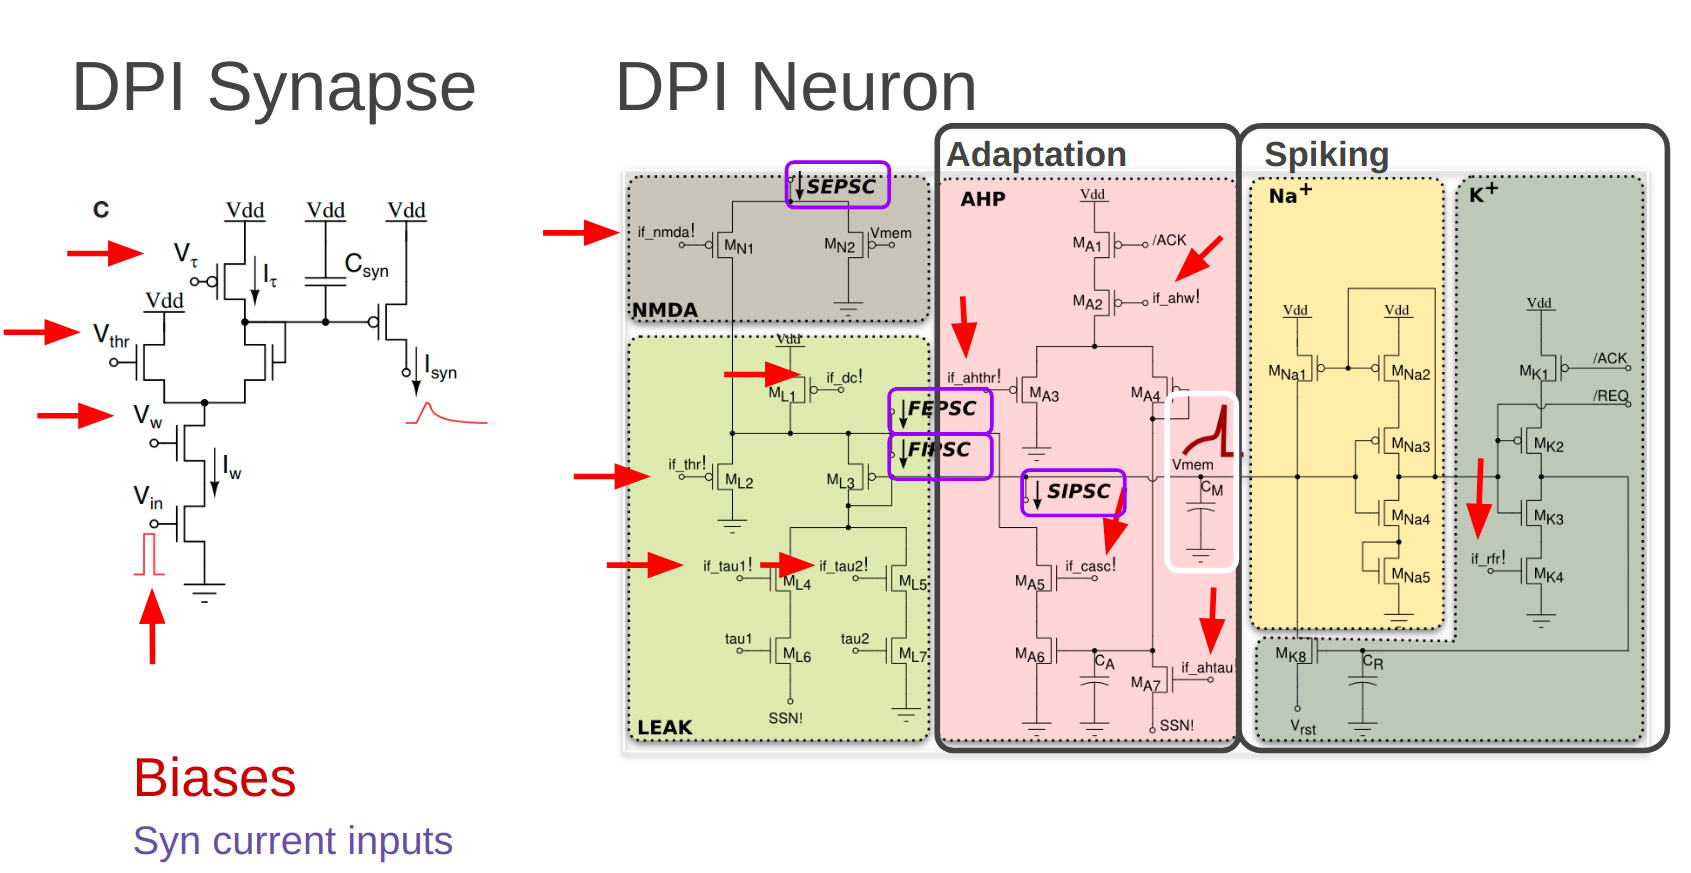
\includegraphics[width=\textwidth]{img/chapter4/DPI_neuron_and_synapse.png}
    \caption[Schematics of circuits of a DPI \ac{ADEXP-LIF} neuron and a DPI alpha synapse]{Schematics of circuits of a DPI \ac{ADEXP-LIF} neuron and a DPI alpha synapse, adapted from~\cite{Chicca_etal14, Livi_Indiveri09}. All transistors are operated in the subthreshold regime, with circuits emulating the synaptic current and the voltage shape on their output nodes, respectively. Red arrows highlight gate voltages controlling behaviour properties of the neuron and the synapse, such as the time constants, refractory period or synaptic weights.}
    \label{fig:DPI_neuron_and_synapse}
\end{figure}

Within these circuits, all neuron and synapse parameters are controlled by gate voltages, or biases, on specific transistors (highlighted in red).

%\dz{TBA: about current-based emulation of parameters? to link to the equations in the next chapter?}

Following~\cite{Chicca_etal14}, the neuron circuit shown in Figure~\ref{fig:DPI_neuron_and_synapse} gives a current-based differential equation, following the form of the original \ac{ADEXP-LIF} neuron Equation~\ref{eq:AdEx} with a few extra terms, but with the membrane voltage of the model is emulated by a current $I_{mem}$: %\dz{TBA: label nodes in the figure, add $GABA_a$ current to the equation.}

\begin{eqnarray}
    \left(1+\frac{I_g}{I_{mem}}\right)\tau_m\frac{dI_{mem}}{dt}&=&-I_{mem} \left( 1+\frac{I_{ahp}}{I_\tau} \right) + \frac{I_g}{I_{\tau}}(I_{in} - I_{ahp} - I_{\tau}) + f(I_{mem})
    \label{eq:dynapse_LIF}\\
    \tau_m & \triangleq & \frac{CU_t}{\kappa I_{\tau}}
    \label{eq:dynapse_LIF_TC}
\end{eqnarray}

where $I_{mem}$ is the state variable representing the membrane potential; $I_{ahp}$ is the firing threshold adaptation current behaving similarly to Eq.~\ref{eq:LIF_adaptation}; $I_{g}$ is the DPI gain current; $\tau_{m}$ is the time constant inversely proportional to the leak current $I_{\tau}$; $f(I_{mem})$ is the positive exponential feedback term and $I_{in}$ is the total input current. The currents $I_{g}$ and $I_{\tau}$ are directly controlled by the respective constant voltage biases \verb|if_thr!| and \verb|if_tau1!|, other biases are also constant but applied indirectly.

If the DPI gain $I_{g}$ is low, the equation can be further simplified under the assumption that $I_{g} \ll I_{mem}$ which brings it closer to the original mathematical model:

\begin{eqnarray}
    \tau_m\frac{dI_{mem}}{dt}&=&-I_{mem} + \frac{I_g}{I_{\tau}}I_{in} + f(I_{mem})\\
    \label{eq:dynapse_LIF}
\end{eqnarray}

\begin{figure}[h]
  \centering
  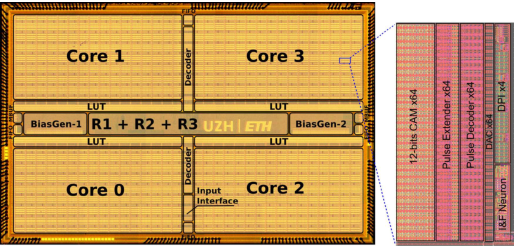
\includegraphics[width=0.75\textwidth]{img/chapter4/chip-dynap-se-pixel.pdf}
  \caption[Die photo of the DYNAP-SE multi-core neuromorphic processor]{Die photo of the DYNAP-SE multi-core neuromorphic processor, with single neuron element highlighted.
The chip was fabricated using a standard 0.18\,$\mu m$ 1P6M \ac{CMOS} technology.
Neurons between cores and between different chips can be interconnected by programming the on-chip CAM memory cells and the asynchronous digital routers labelled R1, R2, and R3.
The circuit parameters can be set independently for each core using on-chip 12\,bit bias generators. Figure adapted from~\cite{Moradi_etal18}.}
  \label{fig:dynapse}
\end{figure}


A circuit producing the synaptic current $I_{syn}$ (also presented in~\cite{Chicca_etal14}) has a similar, albeit simpler (without having the spike generation mechanism) structure, consisting of a pFET DPI, the main capacitor representing the state of the synapse (fully charged meaning there is no synaptic current), the leakage current $I_{\tau_{syn}}$ controlling the synaptic pulse relaxation, and a spike processing branch producing an instantaneous change to the capacitor voltage with the current $I_w$ with fixed amplitude, modelling the synaptic weight, whenever an input event opens the $V_{in}$ gate. The equation for $I_{syn}$ derived from the circuit (Figure~\ref{fig:DPI_neuron_and_synapse} left) is the following:

\begin{eqnarray}
    \tau_{syn}\frac{dI_{syn}}{dt}&=&-I_{syn}+\frac{I^{syn}_{g}}{I_\tau} I_w
    \label{eq:DPI_synapse}
\end{eqnarray}

where $I^{syn}_{g}$ is the \ac{DPI} threshold of the synapse circuit, or the synaptic current gain.

Utilizing these circuit designs, a \ac{DYNAP}-SE1 chip had been created~\cite{Moradi_etal18}, containing 1024 of these silicon neurons placed on the same die (see Fig.~\ref{fig:dynapse}), allowing the circuits to emulate neuronal dynamics completely independently for all neurons, achieving ultimate asynchronous parallelism. 

On this chip, every neuron has 4 synapse circuits attached to the neuron circuit, implementing 4 different synapse types by injecting or subtracting synaptic currents from the neuron at various points (marked in purple on the neuron circuit in Figure~\ref{fig:DPI_neuron_and_synapse}). The FEPSC ("fast excitatory postsynaptic current") and FIPSC nodes are the "fast" excitatory ($AMPA$) and inhibitory ($GABA_B$) synapses, modelling additive and subtractive (dendritic) synaptic inputs, respectively. The SEPSC ("slow" EPSC) is connected through an extra \ac{DPI} circuit, enabling the $NMDA$ voltage gating. Without the $NMDA$ bias (shown as \verb|if_nmda!| in Fig.~\ref{fig:DPI_neuron_and_synapse}), this synapse functions identically to $AMPA$, allowing having two excitatory synapse types for the neuron with individual parameter control (as the biases for each neuron and synapse are shared across the core for bias generator chip area reasons, as discussed before). Finally, the SIPSC (or $GABA_A$) node is the somatic inhibition, subtracting charge directly from the neuron capacitor.

The implemented architecture allows direct monitoring of the neuron's capacitor voltage $V_{mem}$ with the oscilloscope, allowing probing of individual neurons, which is heavily utilized throughout this work.

\newpage
\section{The precise, the hidden and the complex. The Triangle of uncertain relations (between model, hardware and chip-derived neuron implementations)}
\label{subsec:triangle_of_relations}

Having discussed the details of the mathematical neuron models and the silicon circuits that implement them, we arrive at the problem of configuring the neuron parameters to produce consistent behaviour across the domains (as illustrated in Figure~\ref{fig:triangle_of_relations}).

\begin{figure}[h]
  \centering
  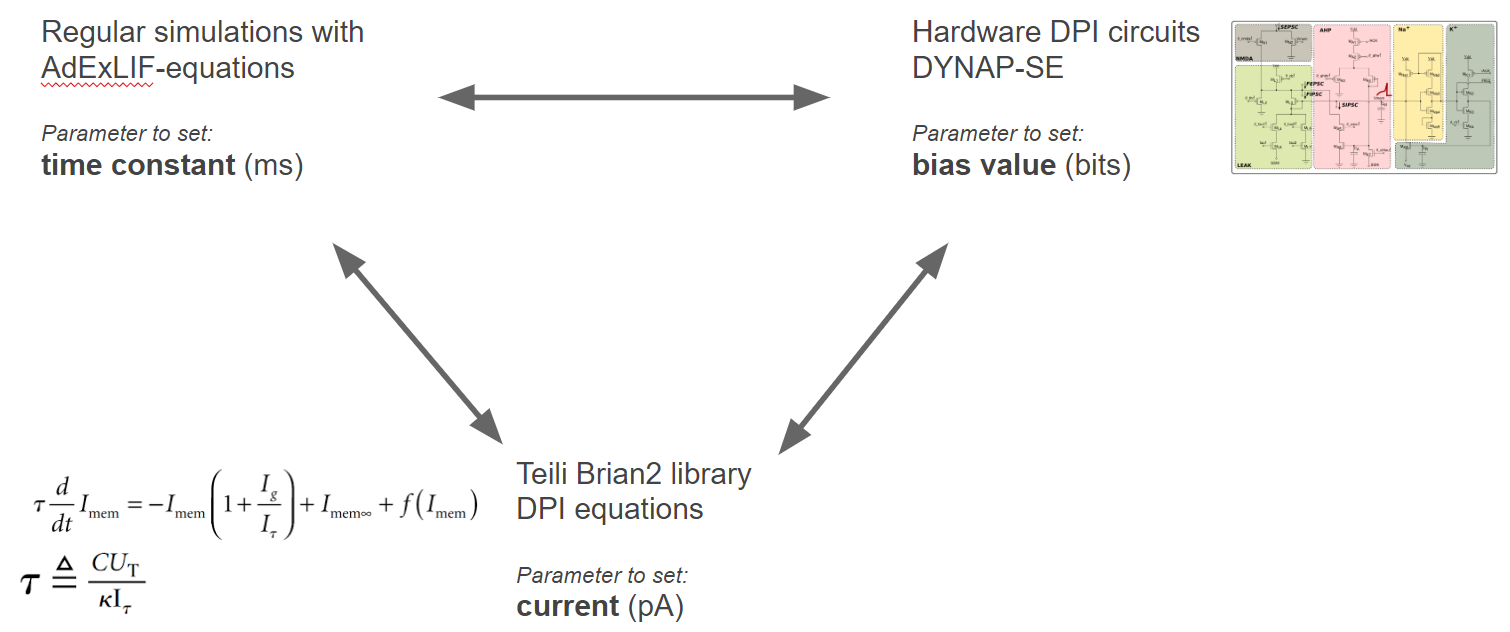
\includegraphics[width=.9\textwidth]{img/chapter4/Triangle_of_uncertainty.png}
  \caption[The problem of mapping between the three domains of modeling spiking neuron dynamics.]{The problem of mapping parameters between the three domains of modeling spiking neuron dynamics: (i) the simulation of the true AdExLIF neuron equations, (ii) the hardware silicon neuron and (iii) the circuit-derived silicon neuron equations~\cite{Milde_etal18}. For the example of a neuron time constant, in all three cases the parameters to set a different: the time constant in units of time, the bit string for the bias generator or the leakage current, respectively. While the link between the two types of simulations can be bridged by approximating the time constant from the transistor equation, a mapping the hardware is impossible to define due to unobservable variability of not only neuron circuits but also the bias generators.}
  \label{fig:triangle_of_relations}
\end{figure}

For the example of the neuron time constant, in numerical simulations of Equation~\ref{eq:AdEx} it is directly set as a parameter $\tau_m$ in the units of time, while for the case of the on-chip current-based DPI neuron circuit, the value controlling the neuron time constant is an abstract \emph{bias value} that is interpreted by the bias generator block, that in turn controls the membrane leakage current.
And completely apart from the two, in a numerical simulation package~\cite{Milde_etal18}that uses the hardware-derived equation (Eq.~\ref{eq:dynapse_LIF}), the time constant is set by the value of the leakage current in pA directly.

To connect the three domains together, there needs to be a precise calculation of a bias current produced by the bias generator on hardware and the corresponding calculation of a resulting neuron parameter. This mapping is, in fact, a big challenge to define, as the bias generator circuit itself is a subthreshold circuit~\cite{Delbruck_etal10} is subject to silicon variability, and the real bias current on the chip cannot be measured directly.

The DPI neuron Equation~\ref{eq:dynapse_LIF} sits in the middle of the three in terms of the neuron dynamics complexity: it has more nonlinear interdependent variables compared to \ac{ADEXP-LIF} Eq.~\ref{eq:AdEx}, but is itself only an approximation of the physical processes happening in the silicon circuit (i.e. not capturing the effects when certain transistors go in/out of saturation).

The strategy we use to bridge the simulation and the emulation domains closer together is the measurement and the response waveform analysis of the silicon neurons through the only available analog state parameter $V_{mem}$. Through such measurement automation we can build the maps between the bias values and the parameters set to the circuit. The same can be done by fitting the simulation traces to confirm the proportionality factor of the Equation~\ref{eq:dynapse_LIF_TC}. But before we do that, however, we need to address the built-in variability of the subthreshold silicon circuits, as the same bias value results an in a distribution of the on-chip neuron behaviours.

%\subsection{Subthreshold circuits. Simulation and emulation.}

%\dz{REWRITE:  is truly a beautiful invention. It gave rise to the entire industry of digital computation as a space- and energy-efficient logic gate, and it kept on giving.}\\

%This section gives a brief and work-relevant introduction of the \emph{neuromorphic engineering} field, the approach of utilizing the physics of subthreshold analog \ac{CMOS} circuits to directly emulate the bio-physics of spiking neurons and synapses through device physics~\cite{Mead90,Mead20}. In conventional electronics, \ac{MOSFET} transistors are normally considered ``closed'' with gate voltage below threshold, as no drift current goes through the channel. The diffusion current that remains if the gate voltage is not equal to the source voltage is usually disregarded, as it depends exponentially on the gate voltage and covers multiple orders of magnitude, which is extremely hard to work with.
%However, exactly this subthreshold behaviour of transistors arranged in a differential pair inspired the association with modeled conductances through the squid neuron cell membrane~\cite{Hodgkin_Huxley52} to create the first silicon neuron circuit~\cite{Mahowald_Douglas91}.

%This idea of emulating mechanisms of one domain by similarly behaving physical properties in the other could be seen as the initial spark, the ground-laying block of the bottom-up ``understanding by building'' approach, where the computation done by biological systems could be studied through reproduction. Having drawn the parallels between exponential behaviour in biophysical processes and diffusion current, the first \emph{neuromorphs} began building circuits emulating the behaviour of the biological counterparts.\\





%\dz{TBA: Add recording for all synapse type shapes here? sharing the synaptic parameters?}

%The communication between the neurons is done via a digital asynchronous hierarchical router~\cite{Moradi_etal18}, with reprogrammable \ac{CAM} and \ac{SRAM} cell located directly at individual neuron circuits, making the \ac{DYNAP}-SE1 chip fulfill the definition of a non-von Neumann mixed-signal processor with truly asynchronous in-memory computing.



%The connectivity solution on this chip is digital but event-driven, meaning that a spike generated by a neuron is immediately picked up by the router \dz{(as soon as it's free to receive an event)~\cite{Moradi_etal18}} and transferred to its postsynaptic neurons based on the reprogrammable \ac{LUT} (i.e. the connectivity matrix), where those events trigger analog current pulses at the input nodes of the synapse circuits.
%This architecture allows to have an efficient, fully parallel real-time emulation of dynamics of a network of \ac{ADEXP-LIF} with a completely flexible connectivity while also \dz{enjoying} the low power consumption aspect of the subthreshold circuits.
%\dz{THIS SECTION NEEDS VERIFICATION FROM THE ROUTING PAPER} The trade-off one faces here is the management of the on-chip surface area. The most area is always taken by capacitors and memory \dz{CHECK THIS}. The decentralized \dz{IS IT?} routing scheme occupies a significant amount of space (around 30\% of the full neuron cell), which is comparable to the area taken by the neuron circuit itself, limiting the fan-out and fan-in of the neuron cells, and thus the reconfigurability of networks the chip can emulate. Another area-induced constraint is the shared parameter setting between the circuits. The bias generators take up a considerable chip area, so in the \ac{DYNAP-SE1} chip design, the bias currents are applied to all 256 neuron cells of a core.



\section{Mismatch and variability in analog neuron circuits. A biological approach to hardware characterization.}

%\dz{This section is adapted from Section 2.2 published in the paper~\cite{Zendrikov_etal23}}.

Having discussed the basics of the neuromorphic circuits we operate with, we need to explore the two other properties inherent to this class of devices.

One is the variations in silicon doping or mismatched geometries intrinsic to the fabrication process of \ac{CMOS} devices~\cite{Pelgrom_etal89} which because of the very low currents (and therefore high sensitivity to such device mismatch) yields heterogeneous electrical properties. These heterogeneous properties affect the behaviour of the analog circuits, even if they have identical geometries at design time.

This factor is central to analog neuromorphic systems, so the computational design built on top has to handle it natively. In the sections below, we discuss the strategies to cope with variability, but first, we build the tools to characterize its scale and behaviour and facilitate the tuning process.

Another property is the parameter configuration flexibility constraints the chip designers have to introduce as a result of optimising the chip area utilization. While the reconfigurable address memory for communication of the neurons is decentralized, it still occupies more than 30\% of the area~\cite{Moradi_etal18}, meaning a limit on the possible fan-in had to be introduced at some level (this is discussed in greater detail in Chapter 4, when we begin connecting neurons together and face that limit). The other significant constraint due to area saving is the bias generator sharing. The bias generator circuits consist of many transistors~\cite{Delbruck_etal10}, so the biasing current has to be shared between groups of neurons. In the case of this chip, every bias is shared between all 256 neurons of a \ac{DYNAP}-SE1 core.

The framework described below aims to automate and systematically configure the \ac{DYNAP}-SE1 chip parameters, while trying to create a methodology general enough to make it transferable to other analog chips utilizing the same circuit design~\cite{Qiao_etal15, Richter_etal24}.


\subsection{Waveform capture and analysis}

To quantify the device mismatch effects in the DYNAP-SE1 circuits accurately, we first defined a set of shared parameters that produce the desired average neuron and synapse behaviours and then systematically measured the circuit responses across all synapse and neuron circuits integrated on the chip.
We automated the data acquisition process using a computer-controlled oscilloscope (see \pyobject{PyScope} in Appendix~\ref{appendix:pyscope}) and measured the analog subthreshold membrane response of the neuron in response to different types of inputs (see the capture and analysis package~\pyobject{BiasTuner} in Appendix~\ref{appendix:bias_tuning_tools}).
We recorded all the measurements on a work-station and carried out standard signal analysis routines to derive the neuron refractory period, the neuron time constant, the synaptic weight and the synaptic time constant from the recordings (see Fig.~\ref{fig:automated_acquisition}).


The refractory period of individual neurons was measured by driving the neuron to produce regular spikes trains with constant input currents, as depicted in Fig.~\ref{fig:neuron_ref}.
The refractory period was defined as the time interval between the action potential reset and the voltage of the neuron rising above the 20\% of its value at rest.

The neuron's time constant was estimated by fitting its response to a step input current small enough to keep the neuron's membrane potential below its firing threshold.
The fit was performed for the decaying part of the circuit response, corresponding to the removal of the input current (see Fig.~\ref{fig:neuron_TC}).

\begin{figure}[h]
  \begin{subfigure}[b]{.3\textwidth}
  \centering
  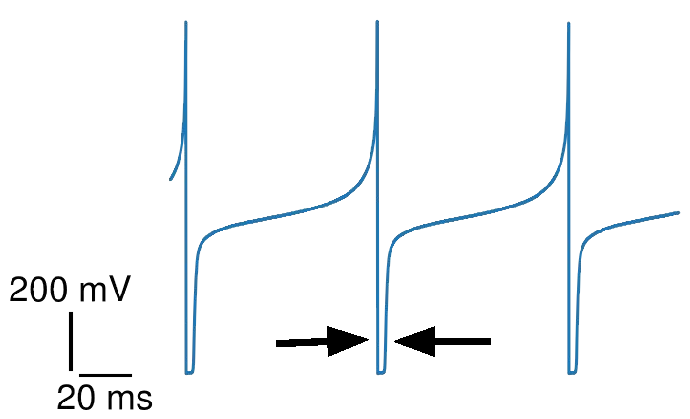
\includegraphics[width=\textwidth]{img/chapter4/neuron_ref.pdf}
  \subcaption{}
  \label{fig:neuron_ref}
  \end{subfigure}
  \begin{subfigure}[b]{.34\textwidth}
  \centering
  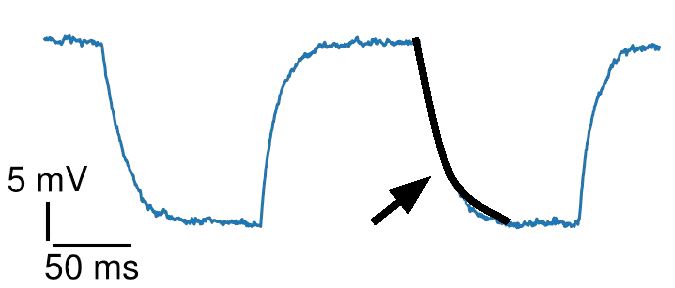
\includegraphics[width=\textwidth]{img/chapter4/neuron_TC.pdf}
  \subcaption{}
  \label{fig:neuron_TC}
  \end{subfigure}
  \begin{subfigure}[b]{.34\textwidth}
  \centering
  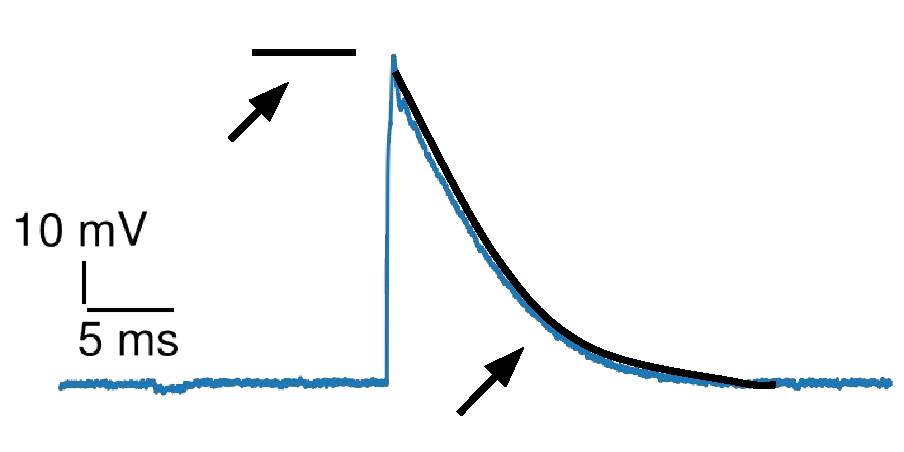
\includegraphics[width=\textwidth]{img/chapter4/ampa_tc.pdf}
  \subcaption{}
  \label{fig:ampa_tc}
  \end{subfigure}
  \caption[Automated measurement of neuron and synapse silicon circuit properties]{Automated measurement of neuron and synapse silicon circuit properties.
(\subref{fig:neuron_ref}):~Measurement of the refractory period of a neuron responding to constant input DC current.
(\subref{fig:neuron_TC}):~Measurement of neuron membrane time constant by fitting the relaxation part of the neuron response after the subthreshold DC current input.
(\subref{fig:ampa_tc}):~Measurement of amplitude (weight) and time constant of an excitatory synapse.}
  \label{fig:automated_acquisition}
\end{figure}

The synaptic weight and time constants of the synapse were estimated indirectly by analyzing the neuron membrane potential using a more elaborate protocol: we first set the neuron time constant to very short values to allow the neuron to follow its input currents faithfully%\dz{TBA: show how this is derived from the DPI equations}
; then, to generate excitatory or inhibitory post-synaptic potentials (EPSPs and IPSPs, respectively), we stimulated the neurons with $20$\,Hz spike trains and analyzed the pulse response decay in-between input spikes (see Fig.~\ref{fig:ampa_tc}). For inhibitory pulses, a constant DC current input was provided.

The weight values were estimated by measuring the PSP amplitude at the onset of the input spike, and the time constant was estimated by fitting the curve with a decaying exponential.

Here, it is essential to note that since the synapse circuit measurements are indirect, the absolute values of weights are not comparable across neurons, as the neuron circuits themselves overlay their variability profile. Those measurements allow, however, balancing EPSPs vs IPSPs within the same core as they interact within the same neuron circuits.

According to the measurements performed, the neuron time constant parameter has a CV of 18\%, and it's refractory period of 8\%.
Similarly, the CV of the synapse time constant ranges between 7\% and 10\% depending on its type (NMDA or AMPA) and the weight parameter from 14\% to 30\%.

\begin{figure}[h]
\centering
  \begin{subfigure}{.32\textwidth}
  \centering
    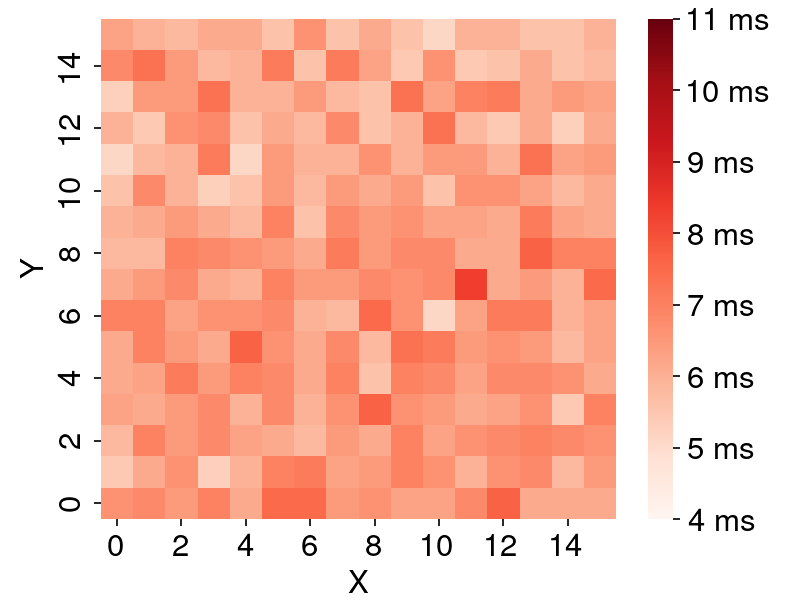
\includegraphics[width=\textwidth]{img/chapter4/rfr_spatial_distribution.png}
    \subcaption{}
    \label{fig:tau_ref_spatial_dist}
  \end{subfigure}
    \begin{subfigure}{.32\textwidth}
    \centering
    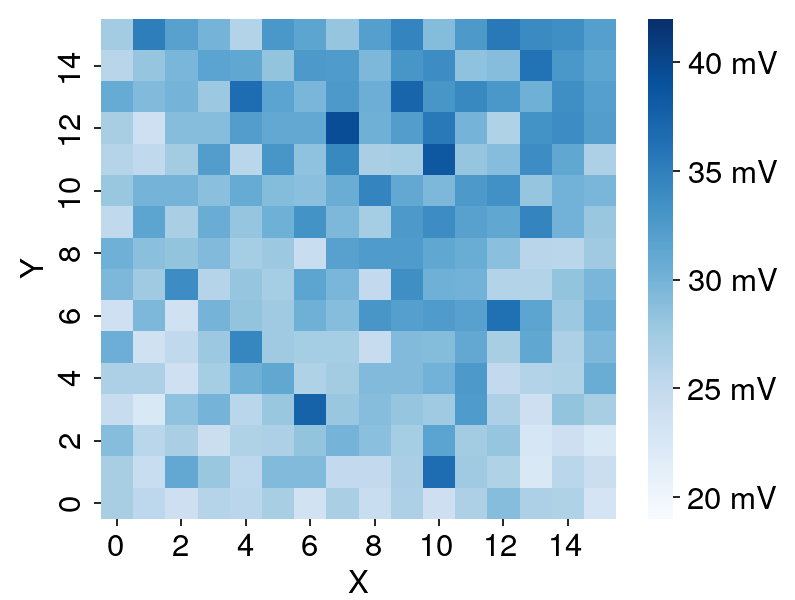
\includegraphics[width=\textwidth]{img/chapter4/wgt_spatial_distribution.png}
    \subcaption{}
    \label{fig:wgt_spatial_dist}
  \end{subfigure}
    \begin{subfigure}{.32\textwidth}
    \centering
    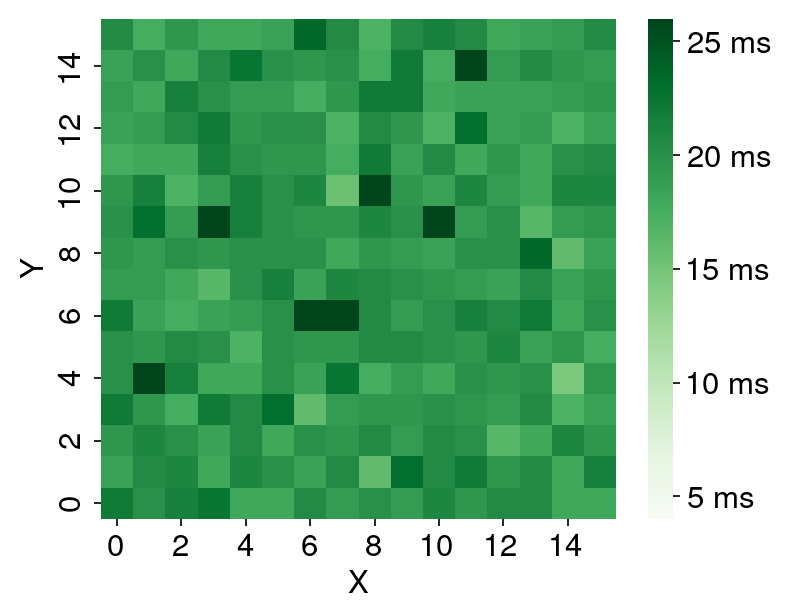
\includegraphics[width=\textwidth]{img/chapter4/tau1_spatial_distribution.png}
    \subcaption{}
    \label{fig:tau1_spatial_dist}
  \end{subfigure}
  \caption[Spatial distribution of mismatch profiles for the neuron and synapse parameters]{Spatial distribution of mismatch profiles for the neuron refractory period (\subref{fig:tau_ref_spatial_dist}), the synaptic weight (\subref{fig:wgt_spatial_dist}), and the neuron time constant (\subref{fig:tau1_spatial_dist}). The $X$ and $Y$ axes represent the neuron id across the layout of the measured core. The measurements were taken for the main fixed set of parameters used to obtain the results.}
  \label{fig:core_spatial_mismatch}
\end{figure}

Even though the variability of different parameters can exhibit different spatial distributions across the chip area, as evidenced by the patterns shown in Fig.~\ref{fig:core_spatial_mismatch}, these spatial distributions differ for each parameter and are generally uncorrelated between parameters.

%\dz{TBA: Show proof (correlograms)?}

As a consequence, the superposition of these effects results in a heterogeneous neuron firing behavior that has no particular correlation with the location of the neuron on the chip layout, or with the specific chip used.

\begin{figure}[h]
  \begin{subfigure}{.5\textwidth}
    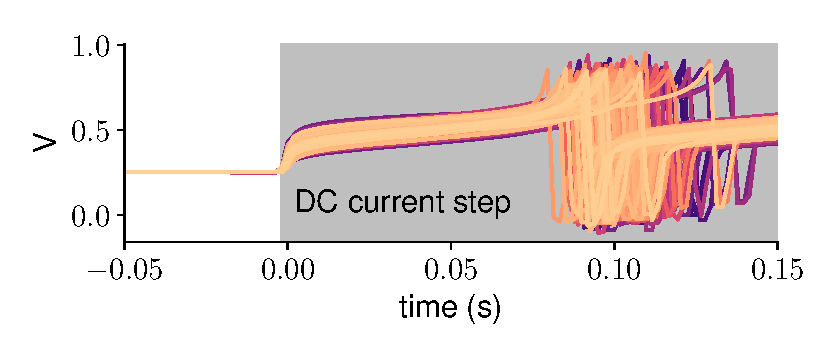
\includegraphics[width=\textwidth]{img/chapter4/ttfs_waveforms.pdf}
    \subcaption{}
    \label{fig:spike_wfs}
  \end{subfigure}
  \begin{subfigure}{.475\textwidth}
    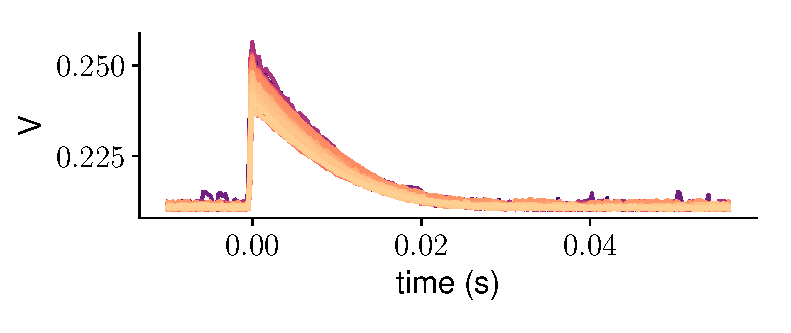
\includegraphics[width=\textwidth]{img/chapter4/epsp_c0c4.pdf}
    \subcaption{}
    \label{fig:epsp_wfs}
  \end{subfigure}\\
  \begin{subfigure}{.5\textwidth}
    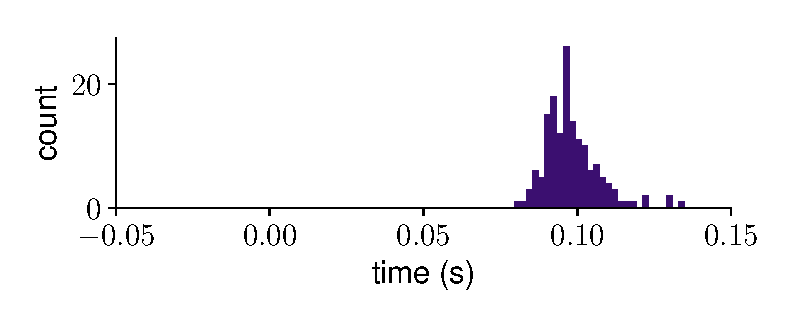
\includegraphics[width=\textwidth]{img/chapter4/ttfs_distribution.pdf}
    \subcaption{}
    \label{fig:ttfs}
  \end{subfigure}
  \begin{subfigure}{.475\textwidth}
    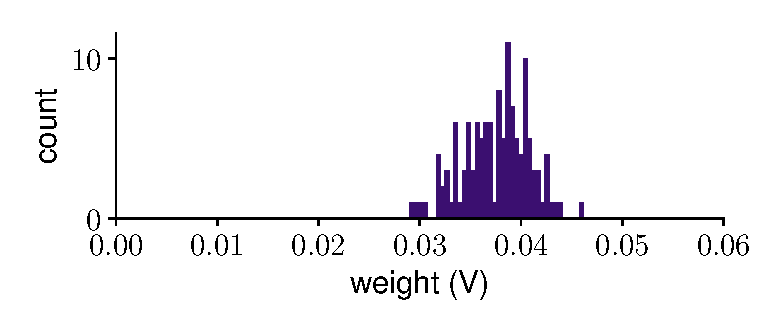
\includegraphics[width=\textwidth]{img/chapter4/epsp_amplitudes_distribution.pdf}
    \subcaption{}
    \label{fig:wfs_dist}
  \end{subfigure}
  \caption[Neuron and synapse variability.]{Neuron and synapse variability.
(\subref{fig:spike_wfs}) Aligned membrane voltage recordings of 256 neuron circuits of one DYNAP-SE core, sharing the same parameters,   in response to a common DC step input current.
Due to device mismatch, the time-to-first-spike of each neuron is distributed normally with CV=9\%; (\subref{fig:epsp_wfs}) Aligned impulse responses of 256 synapse circuits of the same core.
Due to device mismatch the height of the impulse response is distributed around a mean value that is proportional to the same synaptic weight parameter; (\subref{fig:ttfs}) and (\subref{fig:wfs_dist}) show the distributions of the measurements.
  The variation of responses is the cumulative result of individual properties distributions.}
  \label{fig:variability}
\end{figure}


Figure~\ref{fig:variability} shows measurements of such of heterogeneous neuron firing on the DYNAP-SE\@.
For example, when injecting the same input current to multiple instances of \ac{ADEXP-LIF} neurons of one core, the integration and spike generation circuits produce different delays in the time-to-first-spike (see Fig.~\ref{fig:spike_wfs}).
Similarly, when multiple synapses that share the same weight and time constant parameters are stimulated, the device mismatch in these circuits affects the shape of their response (see Fig.~\ref{fig:epsp_wfs}).
When measured across multiple instances of synapse and neuron circuits belonging to the same chip, the response properties of the neuromorphic circuits produce distributions which have typical coefficients of variation (CVs) ranging from 10\% to 20\% (e.g., see Fig.~\ref{fig:ttfs} and Fig.~\ref{fig:wfs_dist}).

%\dz{Requires a table of exact numbers}.

The next section explores how those distributions scale with parameter settings and how this tuning process can be optimized.


\subsection{Setting biases (at scale).}

On the DYNAP-SE1 chip, the parameters neuron and synapse circuits are controlled by bias currents set by 12\,bit temperature-compensated on-chip bias generators~\cite{Delbruck_etal10}.
All 25 available parameters (the main parameters indicated by red arrows in Figure~\ref{fig:DPI_neuron_and_synapse}) are globally shared within a core, and there are four independent bias generators per chip (one per core).

The generated bias current $I_{bias}$ is defined by a 3-bit \emph{coarse} and a 8-bit \emph{fine} values:

\begin{equation}
I_{bias} \approx \textrm{fine}\frac{I_{max}[\textrm{coarse}]}{2^8-1}
\label{eq:bias_current}
\end{equation}
 where


\begin{figure}[t!]
    \begin{subfigure}{.47\textwidth}
    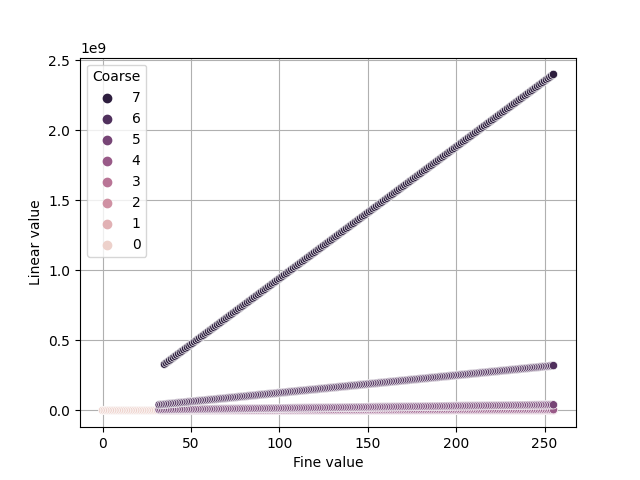
\includegraphics[width=\textwidth]{img/chapter4/linear_bias_map_full.png}
    \subcaption{}
    \label{fig:linear_bias_map_full}
  \end{subfigure}
  \begin{subfigure}{.47\textwidth}
    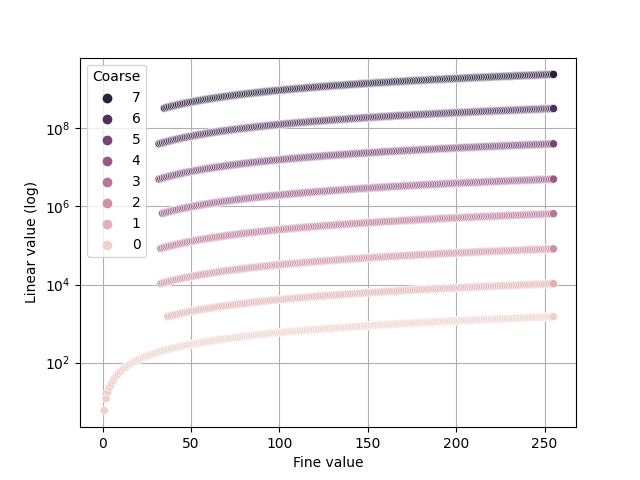
\includegraphics[width=\textwidth]{img/chapter4/linear_bias_map_log.png}
    \subcaption{}
    \label{fig:linear_bias_map_log}
  \end{subfigure}
  \caption[Linear bias value look-up table]{Linear bias value (proportional to the bias current) as a function of the fine and coarse values of the bias generator shown in linear (\subref{fig:linear_bias_map_full}) and logarithmic scale (\subref{fig:linear_bias_map_log}).} 
  \label{fig:linear_bias_map}
\end{figure}

\begin{figure}[b!]
\centering
  \begin{subfigure}{.47\textwidth}
    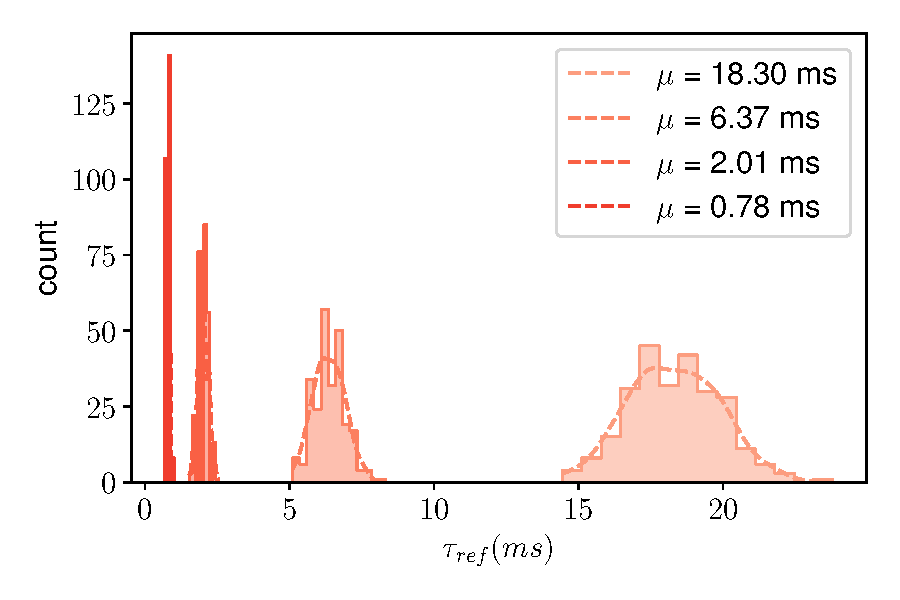
\includegraphics[width=\textwidth]{img/chapter4/scaling_tau_ref.pdf}
    \subcaption{}
    \label{fig:tau_ref_scaling}
  \end{subfigure}
  \centering
  \begin{subfigure}{.47\textwidth}
    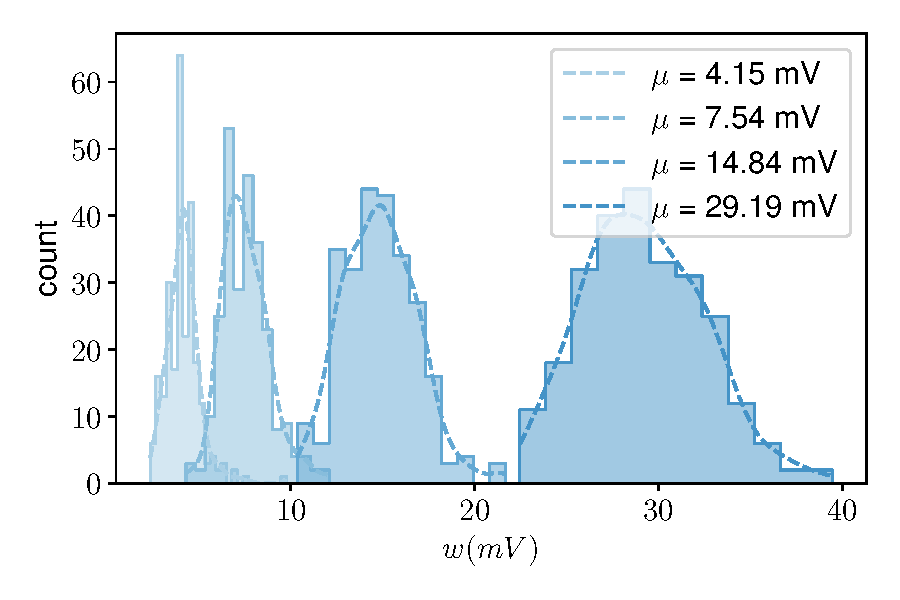
\includegraphics[width=\textwidth]{img/chapter4/scaling_nmda.pdf}
    \subcaption{}
    \label{fig:nmda_wgt_scaling}
  \end{subfigure}\\
  \centering
  \begin{subfigure}{.47\textwidth}
    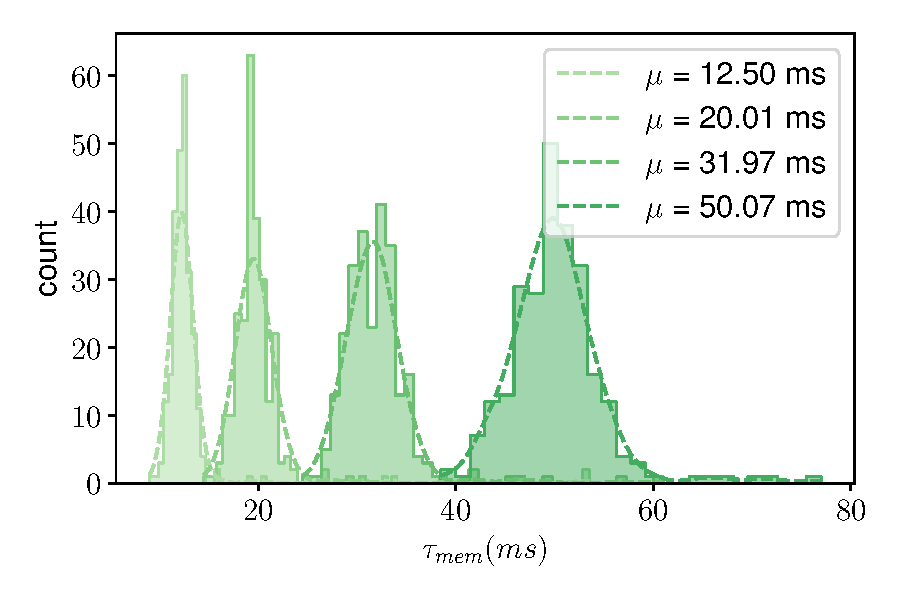
\includegraphics[width=\textwidth]{img/chapter4/scaling_tau_mem.pdf}
    \subcaption{}
    \label{fig:neuron_tau_scaling}
  \end{subfigure}
  \centering
  \begin{subfigure}{.47\textwidth}
    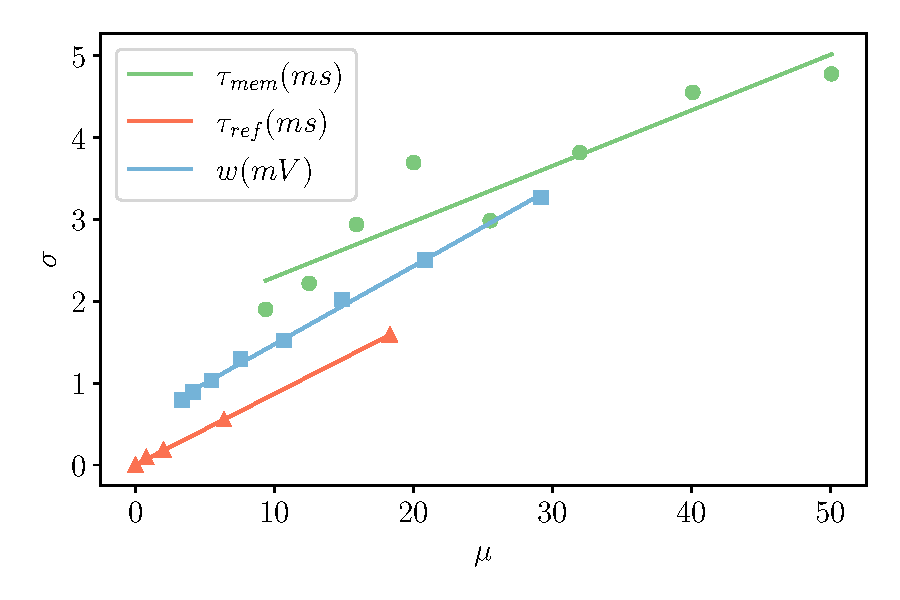
\includegraphics[width=\textwidth]{img/chapter4/scaling_all.pdf}
    \subcaption{}
    \label{fig:bias_CV_scaling}
  \end{subfigure}
  \caption[Variance behaviour across different properties of the DPI neuron circuit (parameter scaling)]{Variance behaviour across different properties of the DPI neuron circuit: (\subref{fig:tau_ref_scaling}) neuron refractory period, (\subref{fig:nmda_wgt_scaling}) synapse weight and (\subref{fig:neuron_tau_scaling}) neuron time constant measured across 256 neurons of the same core for 4 different bias values (shown in shades of the respective color).
  The plot in (\subref{fig:bias_CV_scaling}) shows how the variance changes with the mean, confirming that the CV remains approximately constant for all these parameters.}
  \label{fig:variance}
\end{figure}

 \begin{itemize}
     \item $I_{max} =[15,105,820,6.5 \cdot 10^3, 50 \cdot 10^3, 0.4 \cdot 10^6, 3.2 \cdot 10^6, 24 \cdot 10^6]$ pA
     \item fine $\in [0,255]$, coarse $\in [0,7]$
 \end{itemize}


Note that $I_{max}$ is an estimate and is subject to variability from chip to chip due to mismatch in bias generator circuits. Still, while the Python library \pyobject{samna}~\cite{Samna} used to work with the DYNAP-SE1 chip accepts the coarse and fine bias values, we can use a single continuous \emph{linear} bias parameter that is proportional to $I_{bias}$ and scales continuously between the minimum and maximum current values, to build mappings to physical circuit properties, making the transition to the next \emph{coarse} value when the maximum \emph{fine} value for the current \emph{coarse} value is reached. In Figure~\ref{fig:linear_bias_map_full}, the linear and the logarithmic scales for linear bias values show the graphical representation of such a non-overlapping map. Notable, the higher the $I_{bias}$ current, the lower the precision of it because of the \emph{fine} value discrete step multiplication by the coarse value.

\begin{figure}[t!]
  \centering
  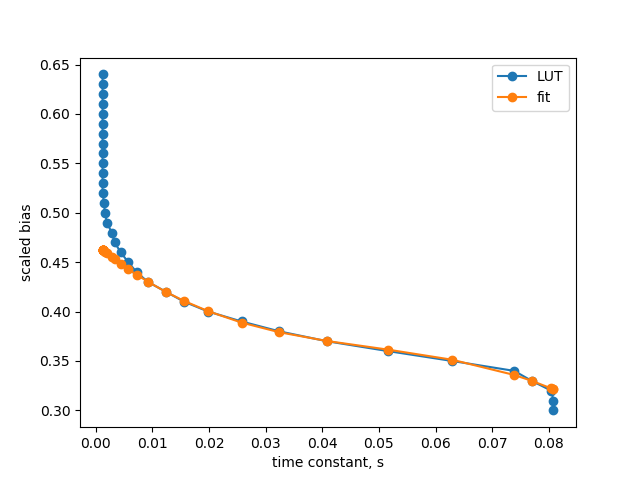
\includegraphics[width=0.8\textwidth]{img/chapter4/Bias_curve.png}
  \caption[Example of a LUT collected for a neuron's time constant]{A map (or a \ac{LUT}, in blue) of a normalized bias value of a neuron membrane leak bias to a mean value of the measured time constant (in seconds) set for the DYNAP-SE1 core. The measurement shows that only a short range of approximately 10\% of the bias values covers the entire range of usable parameter values. A polynomial fit for the usable parameter range is shown in orange, which allows setting interpolated bias values.
  Due to variability, for every core, this range would be shifted.}
  \label{fig:bias_curve_fit}
\end{figure}

Having the automated measurement tools and an understanding of the bias generator, we can start building the mapping between simulation and hardware mentioned in Section~\ref{subsec:triangle_of_relations}.
The final missing piece is the understanding of how the values scale with the bias value.
In Figure~\ref{fig:variance}, we show the detailed distributions of the same three parameters (neuron refractory period, neuron time constant and the AMPA weight) measured across 256 neurons of one core for 4 different values of the bias current for each property.

\begin{figure}[b!]
\centering
  \begin{subfigure}{.6\textwidth}
    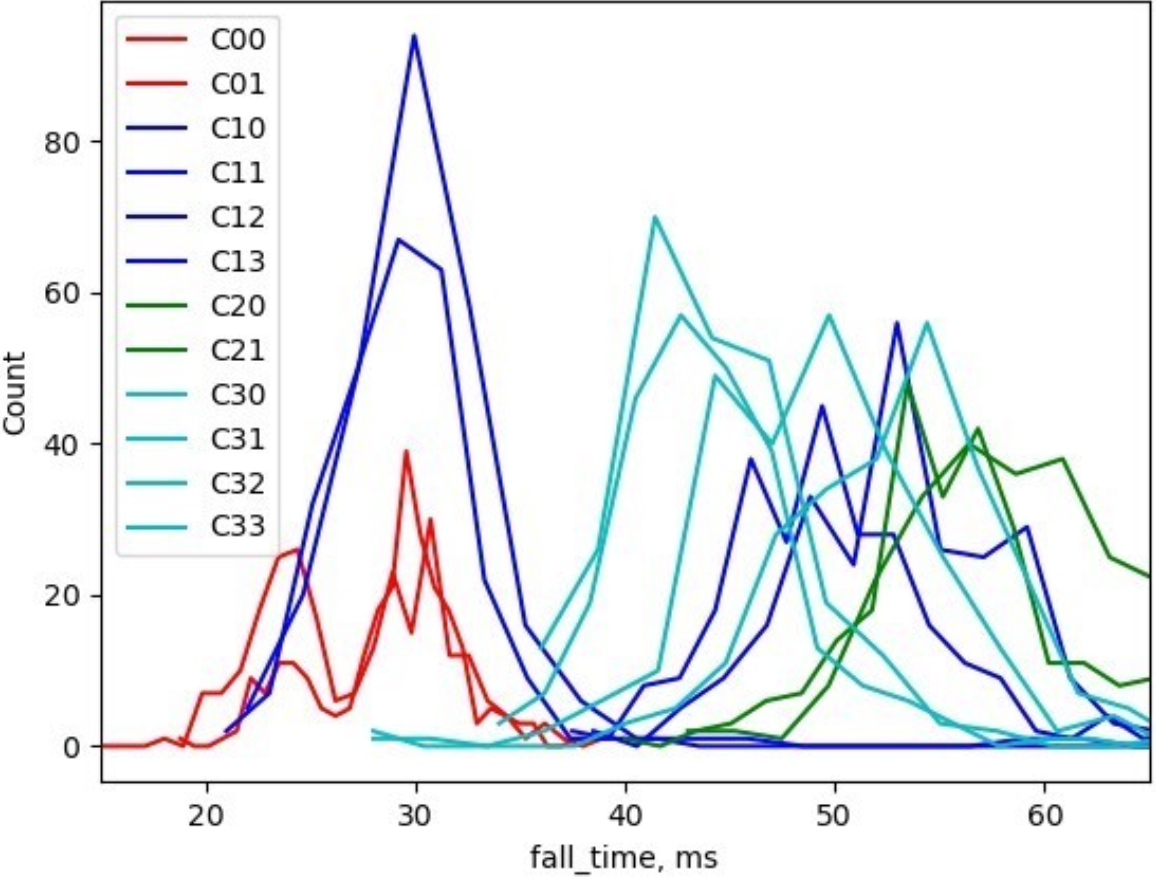
\includegraphics[width=\textwidth]{img/chapter2/cores_TCs_same_bias.png}
    \subcaption{}
    \label{fig:TCs_same_bias}
  \end{subfigure}\\
  \centering
  \begin{subfigure}{.65\textwidth}
    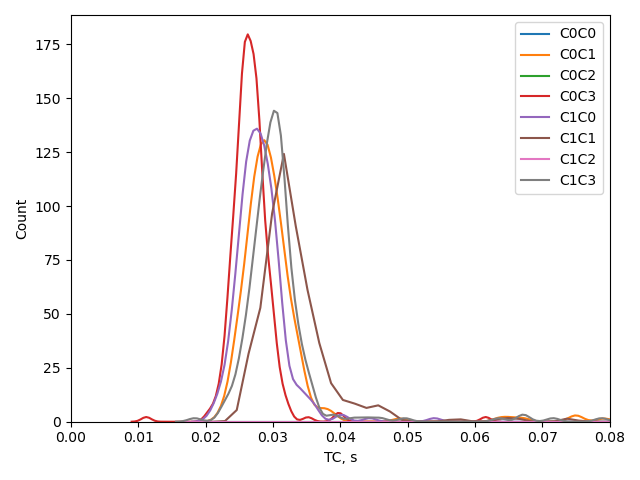
\includegraphics[width=\textwidth]{img/chapter2/taus_tuned_to_30ms_dist_new.png}
    \subcaption{}
    \label{fig:TCs_same_mean}
  \end{subfigure}
  \caption[The result of using the tuning framework to align the time constants across multiple cores of the DYNAP-SE1 chip.]{Tuning the neuron time constant across multiple DYNAP-SE1 cores. Both plots show histograms of distributions of time constants, with one line corresponding to one core of 256 neurons. (\subref{fig:TCs_same_bias}) Result of copying the same bias values across multiple cores. The distributions are located far apart as a result of mismatch both in neuron circuits and in bias generator blocks. Different colours correspond to different chips. (\subref{fig:TCs_same_mean}) Neuron time constant distributions set to a 30ms mean using the LUTs of the \pyobject{BiasTuner} framework. While still not perfectly aligned, the distributions are brought much closer together.}
  \label{fig:TC_tuning}
\end{figure}

As shown in Fig.~\ref{fig:bias_CV_scaling}, the CV of such distributions tends to stay constant across different bias current settings.
This allows to determine exact mismatch measures for individual properties across every core. Specifically, we confirm that the scaling of the properties is uniform, i.e. the neuron with a low time constant compared to the rest of the neurons of the core at a lower bias value would stay at the same part of the distribution for the higher bias value.


Therefore, a tuning strategy optimizing the amount of necessary measurements taken can be proposed. To create a mapping between the bias value and the parameter, a neuron that is close to the \emph{mean} of the parameter distribution can be picked. After the calibration LUT (look-up table) is collected, it can be interpolated within the usable parameter range (see the example for the neuron time constant in Figure~\ref{fig:bias_curve_fit}). Essentially, we pick a single neuron to represent the state of the core for a specific parameter. Note that the range where the parameter takes biologically plausible values is, in fact, narrow (10-15\%) compared to the full possible bias range. This range could be fitted well enough with a polynomial function to interpolate between the measured data points. 

The bias generators, however, are also subject to variability, which explains why the same bias values cannot be just copied between different chip cores. Specifically, Figure~\ref{fig:TCs_same_bias} shows the case when the same bias parameter is copied between multiple cores of multiple dynapse chips. The variability of bias generators defines the locations of means of neuron time constant distributions, while the variability of neuron circuits causes the width of each distribution. On Panel~\ref{fig:TCs_same_mean} these distributions are moved together using the calibration procedure shown in Figure~\ref{fig:bias_curve_fit}, using the interpolated LUTs to set the 30ms means. As a result, the behaviour of the neurons across cores is unified.
\\


\newpage
\section{Averaging across space and time}
\label{sec:averaging}

Spiking neural electronic systems made of high-precision components or ideal neurons in computer simulations represent signals with high fidelity.
In analog circuits, very high levels of precision for representing signals can be achieved only at great costs.
Alternatively, a practical solution, extensively exploited also in the brain, is to relax the high precision constraint for single computational units, the neuron, and to distribute computation in space and time.
Feeding signals to populations composed of heterogeneous units with uncorrelated mismatch in their properties, as in Fig.~\ref{fig:ff_curves}, naturally reduces the effect of noise and variability in the single units.
Averaging signals over time filters out irregularities in the spike sequences generated by both the input sensors and by the neural processing parts of the system.

Figure~\ref{fig:ff_curves} shows the combined effect of both synapse and neuron variability: the plot shows the average firing rate of 16 neurons belonging to the same core, and sharing the same parameter settings.
Each neuron is stimulated via its own excitatory synapse, driven by the same set of input spike sequences of increasing frequency. Although the variability of both synapse and neuron parameters produces response profiles with large differences, the ensemble average response follows the desired profile with good linearity.

\begin{figure}[h!]
\centering
    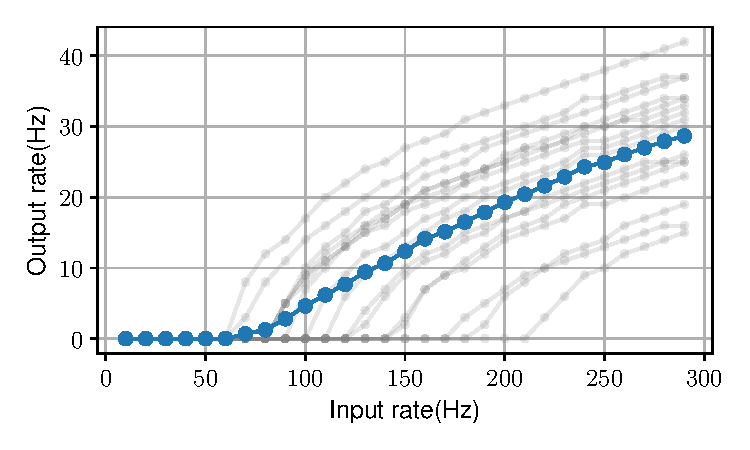
\includegraphics[width=.7\textwidth]{img/chapter4/ff_curves_all.pdf}
  \caption[Variability in transfer functions of 16 silicon neurons.]{Firing rate of 16 silicon neurons belonging to the same core, thus sharing the same parameter settings. All neurons are driven by the same series of regular spike trains with constant rates over one second and step increments of 10\,Hz.}
\label{fig:ff_curves}
\end{figure}

\begin{figure}[h!]
    \centering
    \begin{subfigure}[b]{0.5\textwidth}
        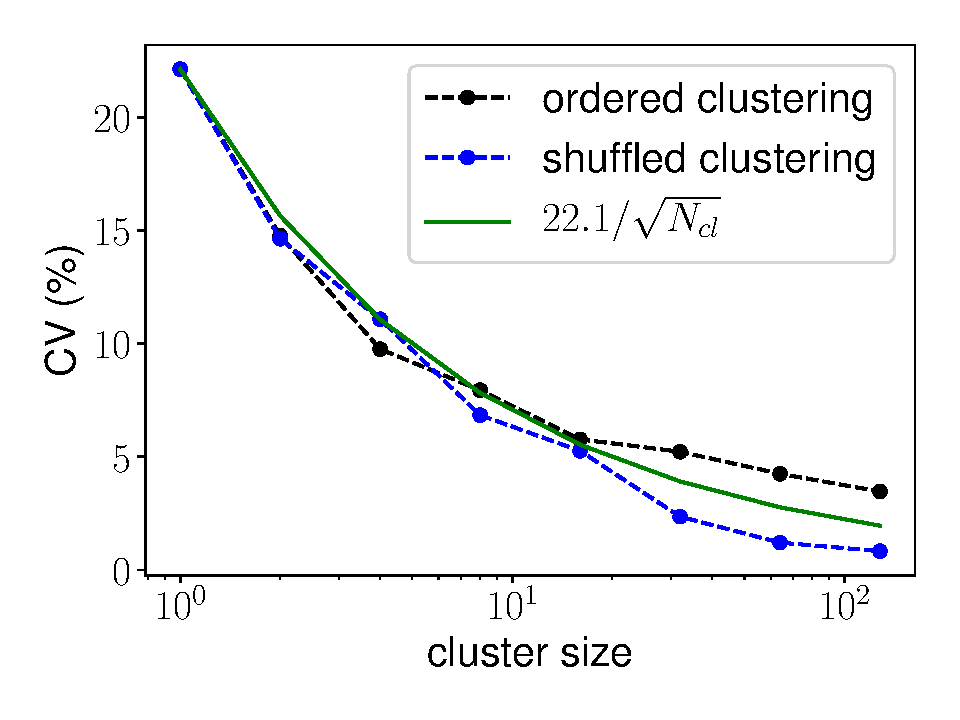
\includegraphics[width=\textwidth]{img/chapter4/CV_clustering_at_50Hz.pdf}
        \caption{}
        \label{fig:variance_vs_cluster_size_a}
    \end{subfigure}\\
        \centering
    \begin{subfigure}[b]{0.7\textwidth}  
        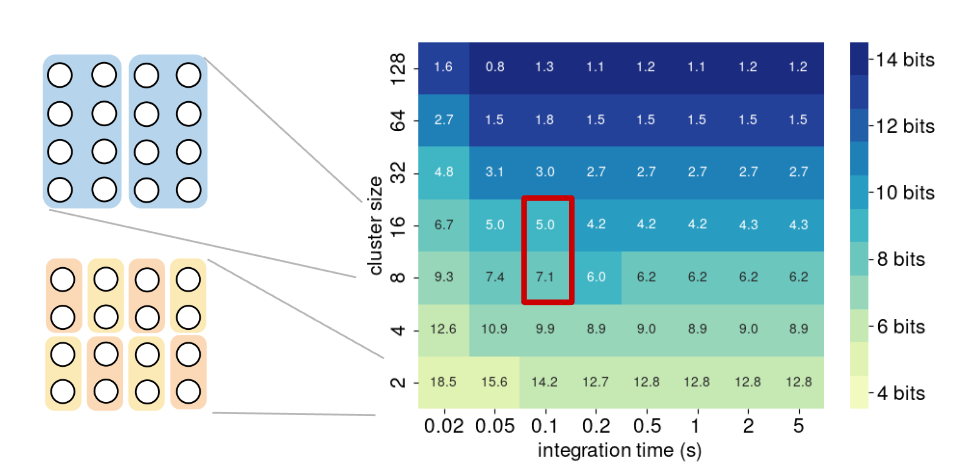
\includegraphics[width=\textwidth]{img/chapter2/Cluster_size_tradeoff.png}
        \caption{}
        \label{fig:variance_vs_cluster_size_b}
    \end{subfigure}
    \caption[Variance of the mean firing rates of clusters of neurons decreases with cluster size]{Variance of the mean firing rates of clusters of neurons decreases with cluster size.
(a): recordings from 256 neurons of the chip with different cluster arrangement (black line for sequential and blue line for randomly shuffled clustering).
All 256 neurons were used at all times, meaning the largest CV is for 256 clusters of size 1, and the lowest is for 2 clusters of size 128.
The green line is a $1/\sqrt{N_{cl}}$ fit normalized to the first value.
The integration time is 1 sec.
(b) Dependence of cluster rate CV (shown in each color coded square) on cluster size (y-axis) and spike integration time (x-axis).
The equivalent bit precision for each CV value is color coded.
Each CV value shown is a mean across 10 random splits (shuffles) into clusters.
Darker color stands for higher precision of encoding.}
    \label{fig:variance_vs_cluster_size}
\end{figure}


The first strategy, of \emph{space averaging encoding}, can be implemented, for example, by feeding the output spike train of one unit to multiple neurons in a cluster.
%(see Fig.~\ref{fig:rate-population}).
We tested this strategy by carrying out an experiment in which a node producing a regular spike train of $200$\,Hz drives a population of 256 neurons, in one DYNAP-SE core, in a way to produce an average output rate of $50$\,Hz.
We computed their individual output firing rates during one second of recording and used its distribution across the cluster to compute the rate CV of different size clusters, ranging from two clusters of 128 neurons to 4 clusters of 64 neurons each, to 8 of 32 neurons, and so on, up to 256 clusters each made of one neuron.
For each combination, the CV of the rate is computed from the mean and variance of the firing rate distribution across clusters, grouping neurons selected within the same single core. 
To measure average values of the CV, we computed the mean CV over $10$ reconstructions of the same configuration with shuffled (regrouped) neurons across clusters.
Figure~\ref{fig:variance_vs_cluster_size_a} shows the firing rate CV computed in this way, as a function of cluster size.
Our data are consistent with the averaging theory, which states that the standard deviation and the coefficient of variation of a distribution is proportional to the $\sqrt{N_{cl}}$, where $N_{cl}$ is the cluster size (see Fig.~\ref{fig:variance_vs_cluster_size_a}).
Thus, the balance between employed resources and acceptable cancellation of mismatch, i.e., firing rate CV reduction, results from a trade-off that scales with $\sqrt{N_{cl}}$.


In the second \emph{time averaging encoding} strategy, the integration time window is a relevant parameter.
Unlike neurons simulated with digital hardware, but very much like biological ones, mixed signal analog/digital silicon neurons produce irregular spike trains even if stimulated with constant inputs, and exhibit heterogeneity in their firing rates across multiple trials even if the input stimulus is always the same.
If we fix an integration bin size, within the same bin, fast firing neurons provide more information than slow ones.
In Fig.~\ref{fig:variance_vs_cluster_size_b}, we estimate the CV for increasing bin sizes, ranging from 20\,ms up to 5\,seconds, calculated for each choice of cluster size.
The trade-off between readout time and amount of resources is now evident: precise rate encoding requires large clusters.
For example, in this experiment an equivalent bit precision of 14\,bits is achieved only by using clusters that comprise 128 neurons.
However, by combining longer integration times (e.g., 100\,ms--200\,ms) with cluster sizes of 8 or 16 neurons it is possible to achieve equivalent bit precision of 8\,bits, which appears to be adequate for many artificial intelligence and neural processing tasks~\cite{Pfeil_etal13,Stromatias_etal15a,Baldassi_etal16}.

An advantage of this approach is that the chip designer does not have to make critical decisions (such as choosing the number of bits to use in a digital bus) at chip design time. The size of the cluster and the integration time can be flexibly changed and even adapted dynamically at run time. 

%\subsection{Population coding as a method to combine rate and space coding}

%\dz{To Be Changed: Move the population coding introduction to here from Chapter 3? Because technically for population coding we do not need to connect any neurons yet.}

%In the array of $N$ input channels, the firing rates would be defined as set the input neuron rates

%\begin{equation}
%    r_i = r_{max} e^{-\frac{1}{2} \frac{(i-\mu-N/2)/N}{\sigma}^2}
%    \label{eq:popcode2rates}
%\end{equation}


\section{Discussion: temperature-induced variability}

In this chapter, we have introduced the systematic device characterization and tuning method. It allowed us to observe the true mismatch profile of multiple DYNAP-SE1 cores in a relatively short amount of time, which was not possible before. This, in fact, allowed to schedule the automated measurement at the different times of day, returning an interesting results shown in Figure~\ref{fig:TC_temperature_variability}.

It shows temperature-induced variability for two measurements taken during the summer day and two at night (of the same day). While the exact temperature delta was not recorded, it should not have changed for more than 10-15C. On the one hand, this measurement aswers how bad the temperature effect really is on the neuron circuits. The answer is that the entire distribution of the time constants can move for almost 1 sigma. On the other hand, this means that our LUTs collected for systematic parameter setting are not that precise: the observed thermal shift would easily convert the requested 30ms time constant into a 25ms one. While this might not look too critical, this is another factor that can through a spiking system out of balance.

\begin{figure}[h]
\centering
    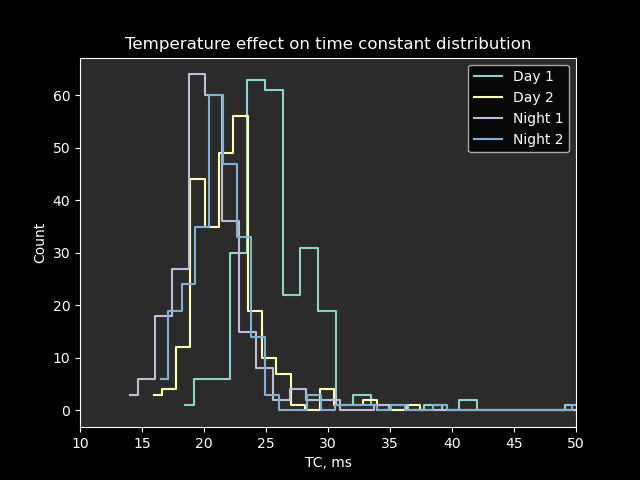
\includegraphics[width=.7\textwidth]{img/chapter2/time_constant_distribution_vs_temperature.png}
  \caption[Temperature dependence illustration]{Distribution of neuron time constants of a single core of 256 neurons of the DYNAP-SE1 chip evolving across multiple days. The distributions might shift by almost one $\sigma$, which is an effect of temperature-induced parameter variability.}
\label{fig:TC_temperature_variability}
\end{figure}

